\chapter{SYSTEM ANALYSIS AND DESIGN}
\section{System Analysis}
As our project code-connect has to be developed in an incremental fashion or it needs to develop step by step with testing the application too. An incremental approach, also known as an iterative or step-by-step approach, is a development or problem-solving method that breaks down a larger task or project into smaller, manageable increments or steps. Rather than attempting to tackle the entire task at once, an incremental approach focuses on making incremental progress by completing and delivering smaller portions of work in a series of iterations.

Here Below are the process that needs to followed
\begin{itemize}
    \setlength\itemsep{0.25em}
    \item Initial Planning and Requirements Gathering
    \item Increment Planning and Design
    \item Development and Implementation
    \item Testing and Quality Assurance
    \item Evaluation and Feedback
    \item Iterative Development and Refinement
    \item Deployment and Release
    \item Repeat the Process for Subsequent Increments
\end{itemize}
\section{Requirement Analysis}
\subsection{Functional Requirements}
The functional Requirements of our project code connect is mentioned below:
\begin{itemize}
    \item \textbf{User Registration/Login}:
      Users will have the option to create an account or log in using their email addresses. This streamlined process ensures that IT professionals can easily access the platform and connect with their peers.
    \item \textbf{User Dashboard/Profile Management}:
      Within the profile management section, users will have the ability to showcase their expertise. Project management enables users to upload and highlight their project details hosted on platforms like GitHub, giving others insight into their skills and contributions. Additionally, Other features allows users to present their skills, experience, and certification in a structured manner. Users can also upload their CV for presentation in their profile.
    \item \textbf{Connection Management}:
      The platform fosters networking by allowing users to send and receive connection requests. This feature encourages the growth of professional relationships and collaboration within the IT community.
    \item \textbf{Discussion/Posts}:
      The discussion and news feed serve as a dynamic space for users to share knowledge, insights, and code snippets. Users can post discussions and engage with others by Geeking on posts, as well as commenting to facilitate meaningful conversations.
    \item \textbf{Messaging (Code Connect Messenger)}:
      The private messaging functionality, known as "Code Connect Messenger," enriches communication. Users can exchange private messages, fostering collaboration, mentorship, and confidential discussions within a secure environment.
    \item \textbf{Notifications}:
      The notifications feature keeps users engaged and informed about interactions on the platform. Users will receive notifications for activities such as receiving 'Geeks' on their posts, receiving comments, and receiving connection requests. This ensures that users stay updated on relevant interactions and stay engaged with the platform's activities.
    \item \textbf{Save/Un-save}:
      This feature allows users to bookmark or save posts or content they find interesting so that they can easily access them later for viewing or reference.

    \item \textbf{Geek/Un-geek}:
      The "Geek/Un-geek" feature, which is similar to the "Like" feature on Facebook, allows users to express appreciation or approval for posts. 

    \item \textbf{Comment/Delete Comment}:
      This feature allows users to add comments to posts and delete their own comments if needed. This will help the users to freely express their point of view on any posts/discussions. 

    \item \textbf{Search Users/Posts}:
    This feature allows users to search other users by their user name and also helps them to find the posts that catches their intrests. This will ensure that the users can easily find other users or posts.

  \end{itemize}
\subsection{Nonfunctional Requirements}
The non functional Requirements of our project code connect is mentioned below:
\begin{itemize}
    \item \textbf{Performance Enhancement}: Our focus on performance involves minimizing reliance on external frameworks and modules. By reducing the use of these components, the aim to streamline the software's execution, resulting in better overall performance and responsiveness.
    \item \textbf{Authentication Security}: Security is a paramount concern. To enhance the platform's security,advanced authentication algorithms, particularly focusing on hashing techniques within the PHP programming environment has been implemented. This ensures that user authentication data is stored and managed in a highly secure manner.
    \item \textbf{Better UX Design}: User experience is central to our project's success. Our emphasis on better UX design means that every aspect of the platform's interface, from navigation to interaction, will be meticulously crafted to ensure a seamless and intuitive experience. This design approach caters not only to experienced users but also to newcomers, ensuring that all users can effortlessly navigate and engage with the platform.
    \item \textbf{Responsive Site}: Recognizing the diverse range of devices and browsers that users utilize, Creation of responsive site is important for this project. This means that the platform's design and functionality will adapt flawlessly to various screen sizes, ensuring that users can access and interact with the platform effectively, whether they are using a desktop computer, tablet, or smartphone. This responsiveness guarantees a consistent and satisfying experience across different devices and platforms, promoting accessibility and usability.
    
  \end{itemize}
\section{Feasibility Analysis}
A feasibility study is a systematic and structured analysis conducted to determine the viability and practicality of a proposed project plan. It serves as an evaluation tool to assess whether the project can be successfully implemented and if it aligns with the project's goals and objectives. It involves gathering and analyzing relevant information to determine if the project is technically feasible, operationally feasible, economically feasible, and scheduling feasible.
\subsection{Economical Feasibility}
Since the system  is a web application, There will be in use of free and open-source software development tools such as HTML,CSS,JS, PHP, MySQL, VS Code and Figma. 
\subsection{Operational Feasibility}
Operational feasibility for the proposed system focuses ease of use. As the system is designed to be interactive, users do not require in-depth knowledge of the web app to navigate and utilize its features. The user interface (UI) is specifically designed to be user-friendly, ensuring a smooth and intuitive experience. This approach minimizes the need for extensive training and reduces potential resistance from users. Even new commers cna use it without any problem or difficulties. 
\subsection{Technical Feasibility}
There are several development technologies available. For frontend development, HTML,CSS,JS is being used. For backend development,  PHP along with the MySQL database is being used. In our application.Here, HTML,CSS,JS, for the frontend and PHP with MySQL for the backend. Both HTML,CSS,JS, and PHP are open-source technologies and are supported by large companies with vibrant communities. This ensures that technical support and resources are readily available. Considering the chosen technologies and their strong community backing, the project is technically feasible.

\subsection{Data Modelling(ER-Diagram)}
An Entity-Relationship (ER) diagram is a visual representation used to model the relationships between various entities in a database. It's a graphical way of showing the structure of a database, focusing on the entities (objects) within the system and how they relate to each other. ER diagrams are widely used in database design and conceptual modeling to help designers and stakeholders understand the data and its relationships.

The figure \ref{ER} is the ER diagram of our system it shows the entities of our database system with their attributes and relationships.Here, User is the main Entity which is connected with many other entites to work for proper functioning of our system. There are different entities which is being used and will be used in further implementations. Different kinds of attribues has been used. This system have relationships like Has,Connects,Posts etc which are crucial part of the system.
\begin{figure}[H]
    \rotatebox{90}{
    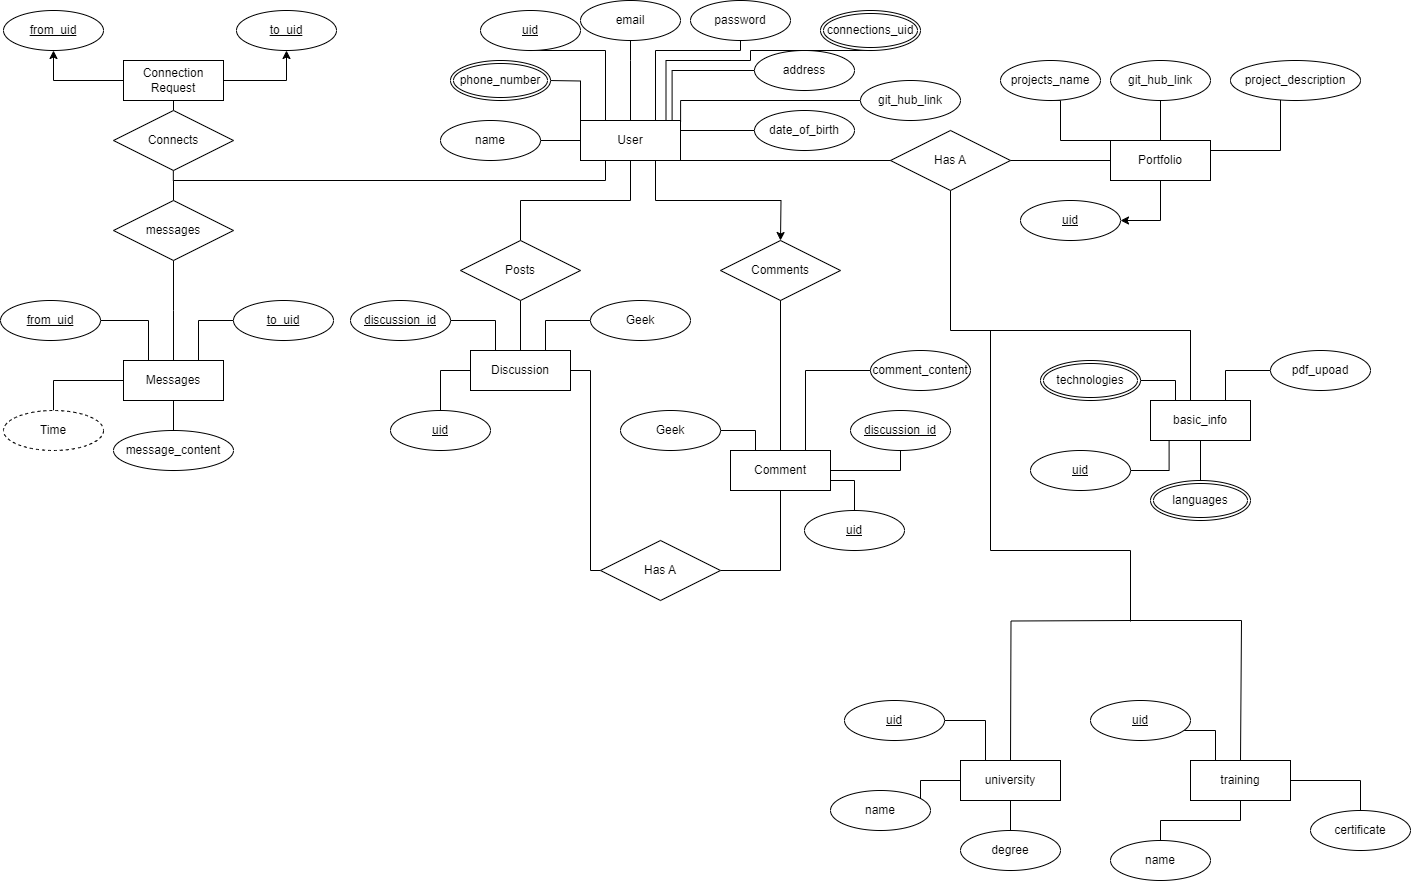
\includegraphics[height = 15cm]{Diagrams/er.drawio.png}}
    \caption{ER Diagram of System Data}
    \label{ER}
\end{figure}
\newpage
\subsection{DFD}
DFD or Data Flow Diagram is mainly used to show how data are being flowed in and out of our system. There are 3 levels of DFD i.e Context Level(Level 0),Level 1 and Level 2, Below is the Context level logical DFD which shows how our program flows data between user and code connect process. Data being flowed with the help of the arrows can be seen.

This diagram helps get brief idea of how our system data flow is going to happen between user and our system.
\begin{figure}[H]
    \centering
    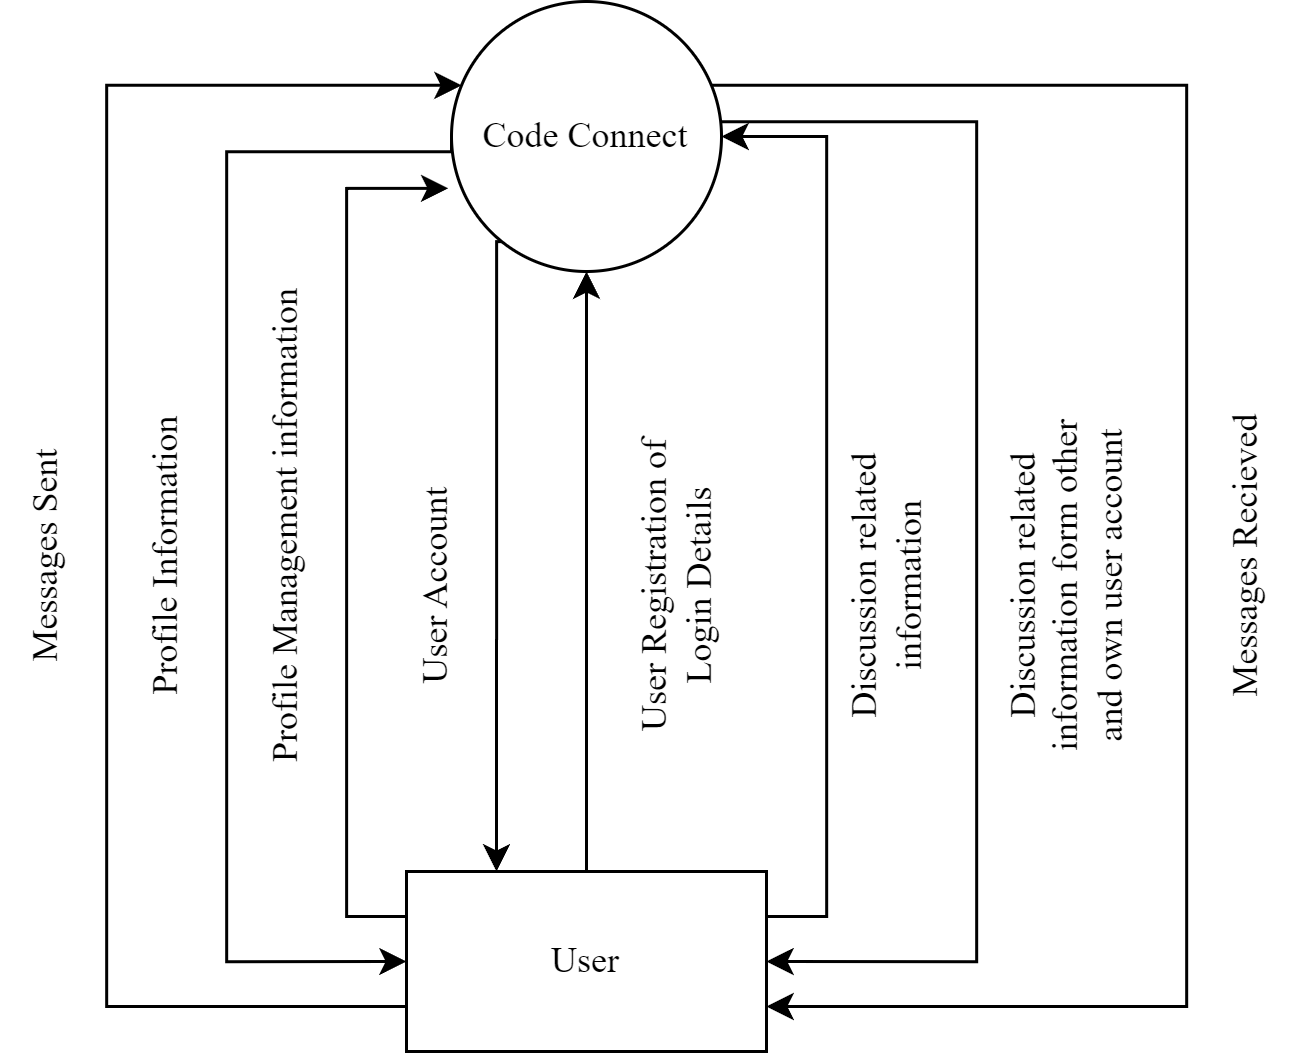
\includegraphics[height = 11cm]{Diagrams/DFD.drawio.png}
    \caption{Data Flow Diagram (Context Level)}
\end{figure}
\newpage
\section{System Design}
\subsection{Architecture Design}
The following diagram shows diagram of our Architecture. Mainly shows what are the functions can be accessed after starting our application.From start users can access different modules to perform their tasks.These are the features and modules that are  being worked on to be implemented. Connection Management, Login/Register Users are fully implemented and other manage discussion is more than half implemented in our system and at last Messaging is being implemented. Manage CV and Portfolio is yet to be implemented.
\begin{figure}[H]
    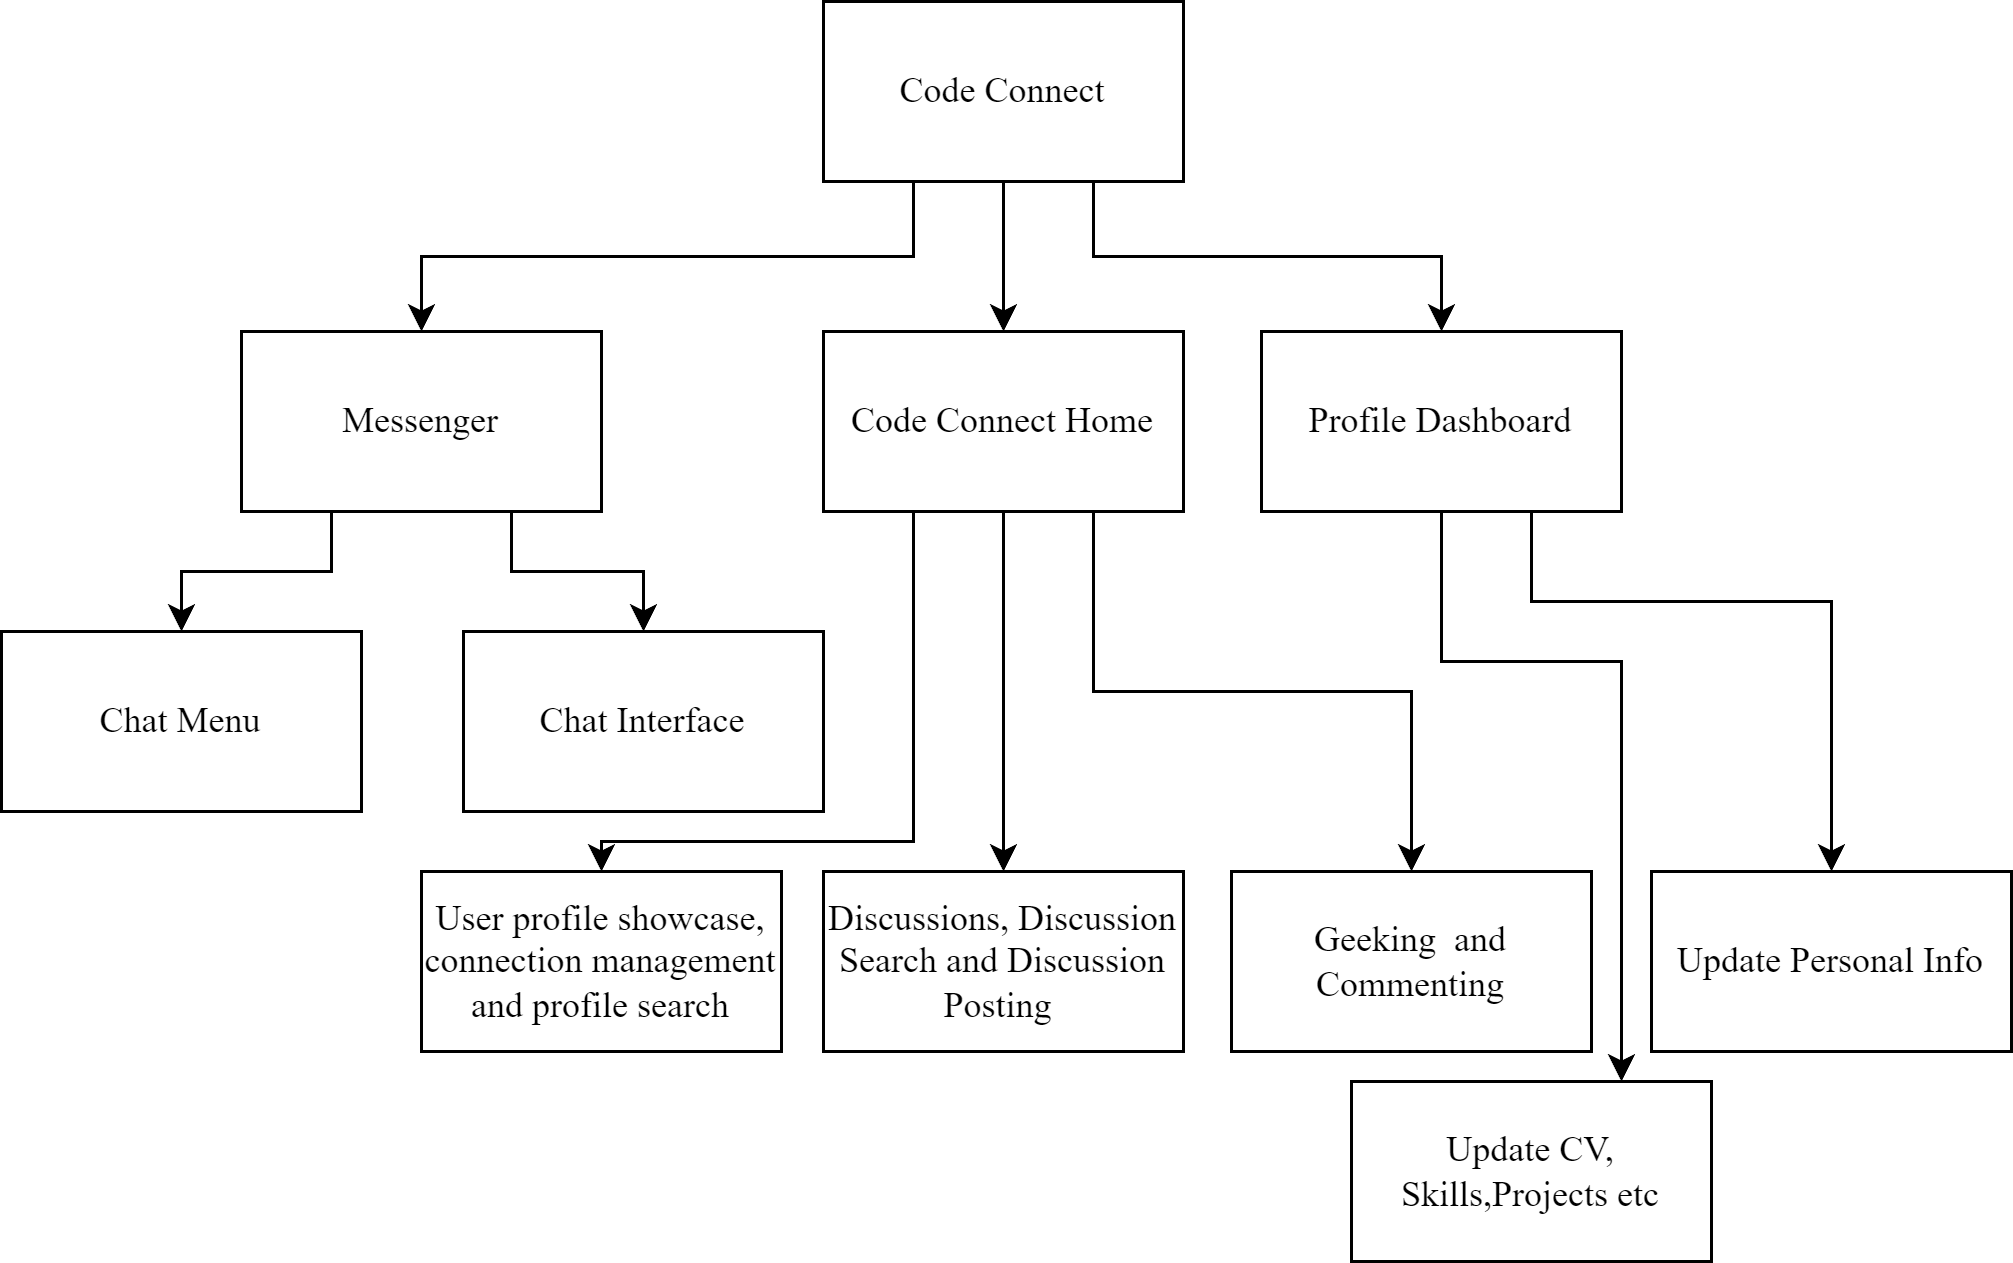
\includegraphics[height = 9cm]{Diagrams/Main_Block.png}
    \caption{Main Architecture of System}
\end{figure}
% \newpage
% \subsection{Activity Diagram}
% An activity diagram visually presents a series of actions or flow of control in a system similar to a flowchart or a data flow diagram. This diagram showed how our program flow goes on. Here it shows how user can go through the process of using our app and what activities they can perform.
% \begin{figure}[H]
%    \centering
%     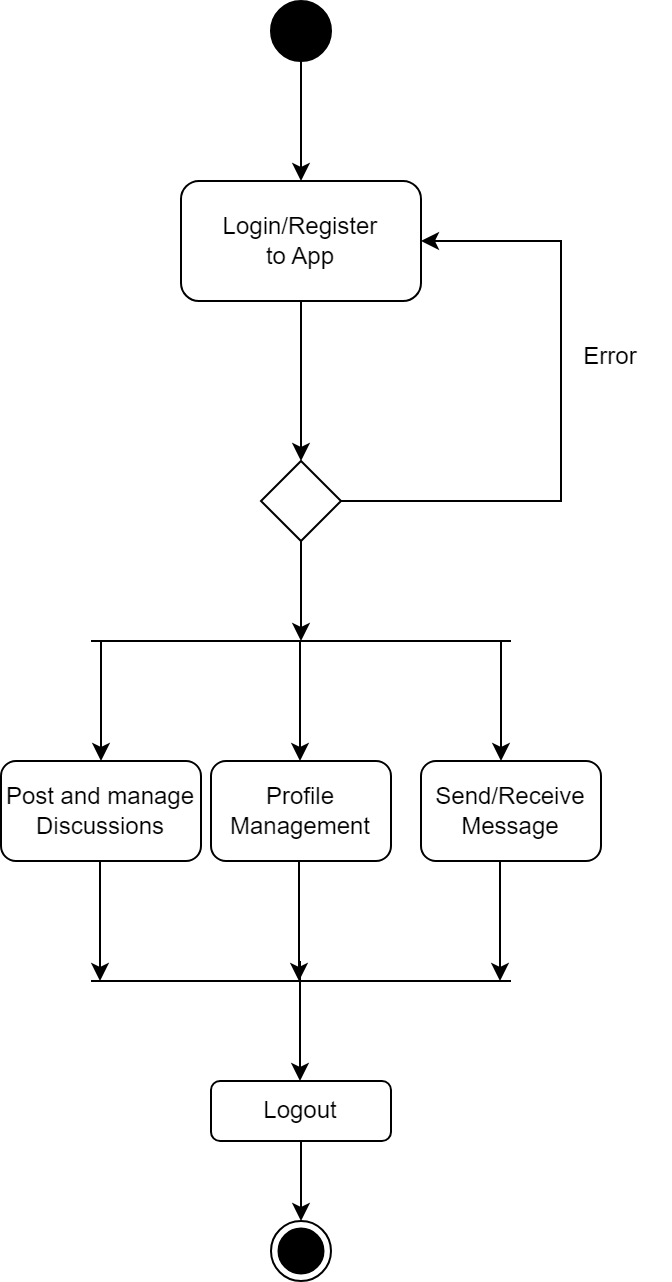
\includegraphics[height = 15cm]{Diagrams/Activity.drawio.png}
%     \caption{Activity Diagram}
% \end{figure}
\newpage
\subsection{Schema Design}
Schema design, in the context of software development and database management, refers to the process of creating a structure or blueprint that defines how data will be organized, stored, and related within a database. It involves making decisions about how different types of data will be represented, how they will be interconnected, and how the database will efficiently retrieve and store information.
\begin{figure}[H]
    \centering
    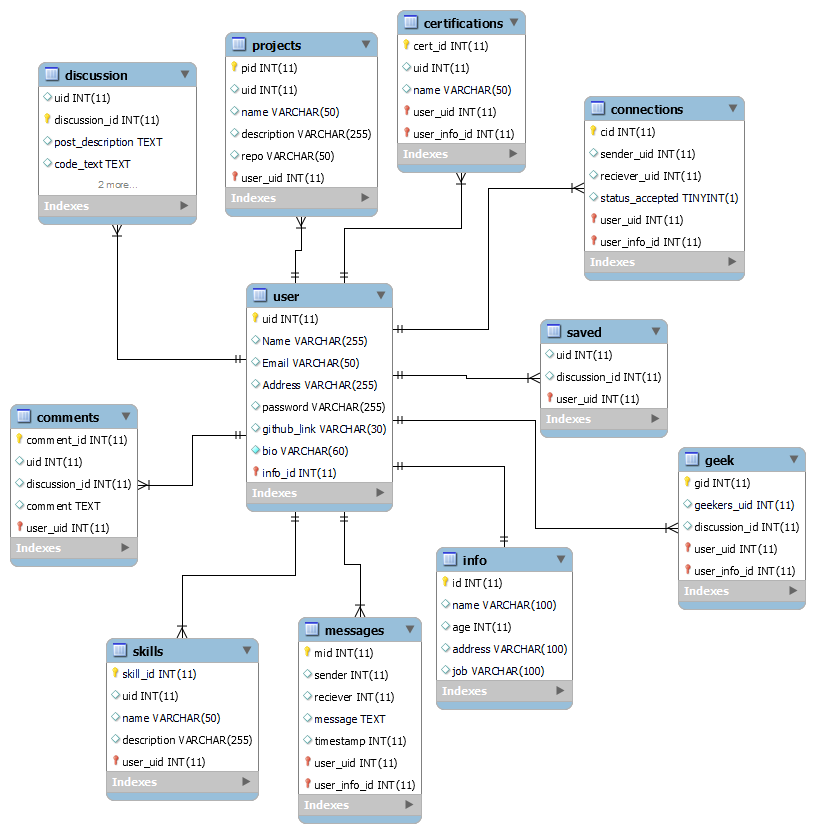
\includegraphics[height = 13cm]{Diagrams/schema.png}
    \caption{Database Schema Design}
\end{figure}
\newpage
\subsection{Interface Design}
\subsubsection{User Interface Design}
User interface (UI) design refers to the process of creating the visual layout and elements that users interact with when using a software application, website, or any digital product. UI design focuses on making the user experience intuitive, visually appealing, and user-friendly. 
\\\\
Below shows the login system UI design which have been implemented in our system.
\begin{figure}[H]
    \centering
    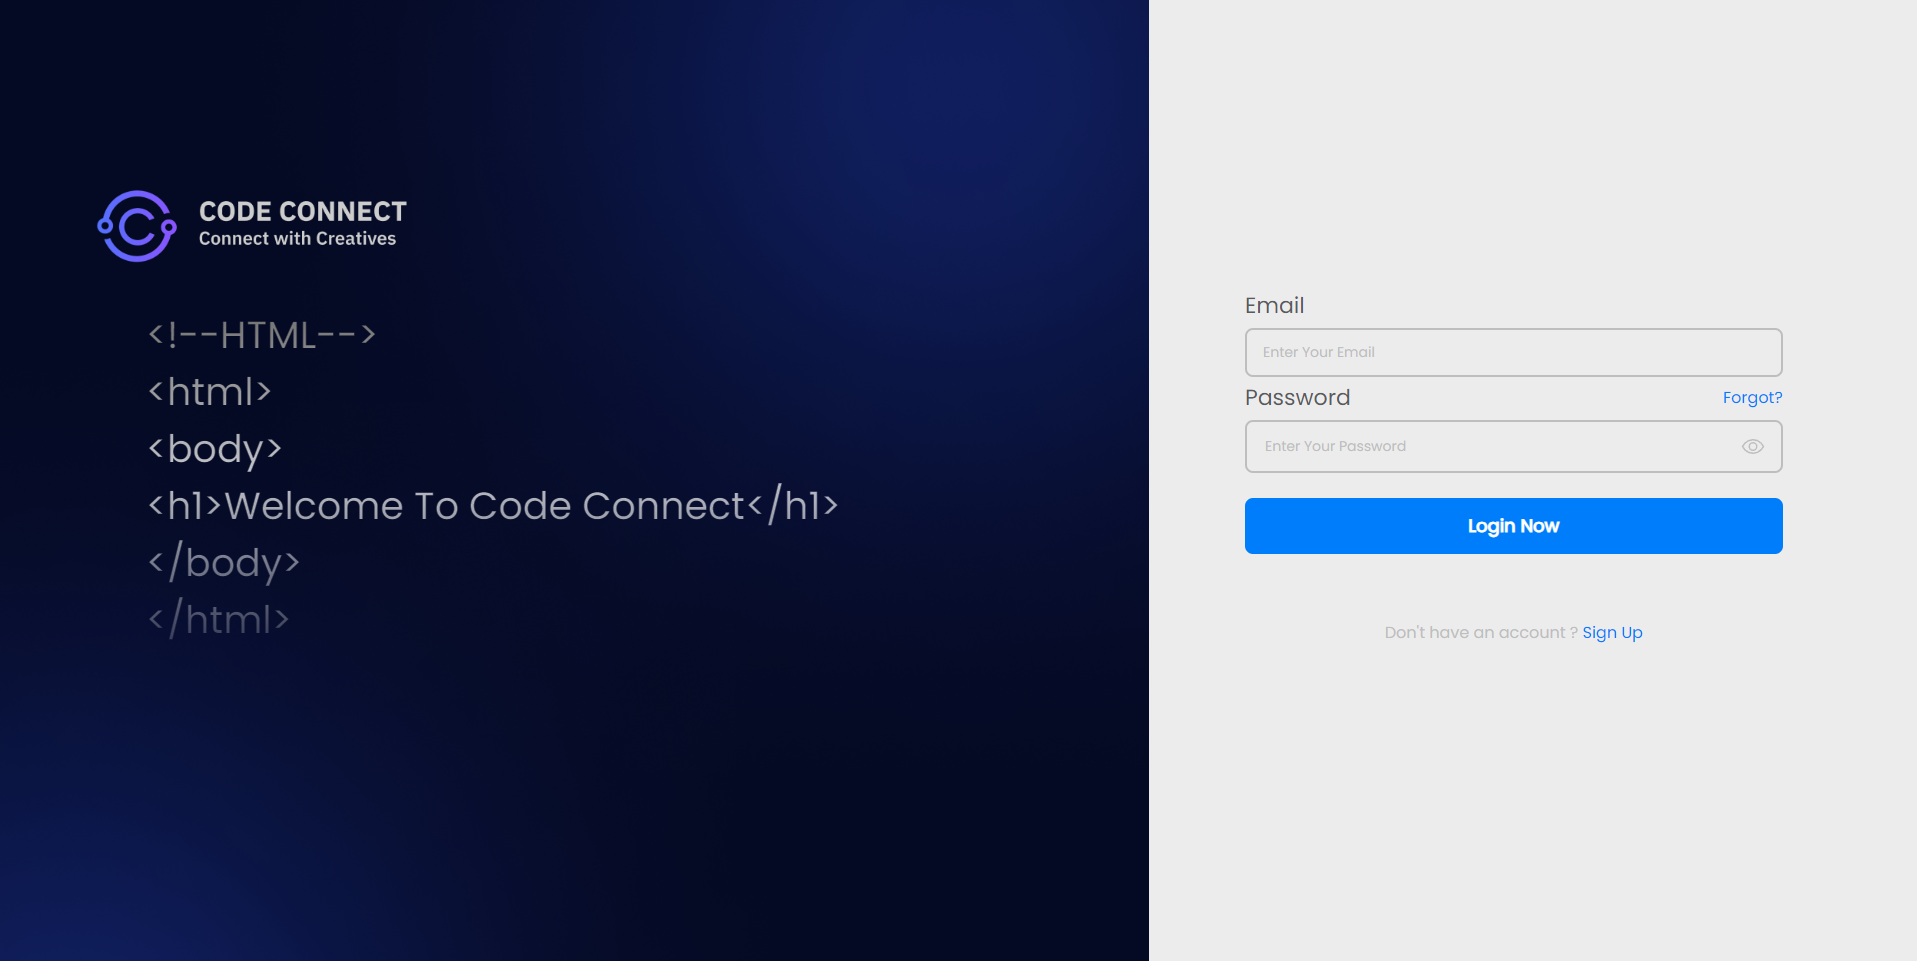
\includegraphics[height = 7cm]{ui_diagrams/desktop_login.png}
    \caption{Desktop Login UI}
\end{figure}
Below is the UI design of our homepage which shows most of our functanilty in our web application.
\begin{figure}[H]
  \centering
  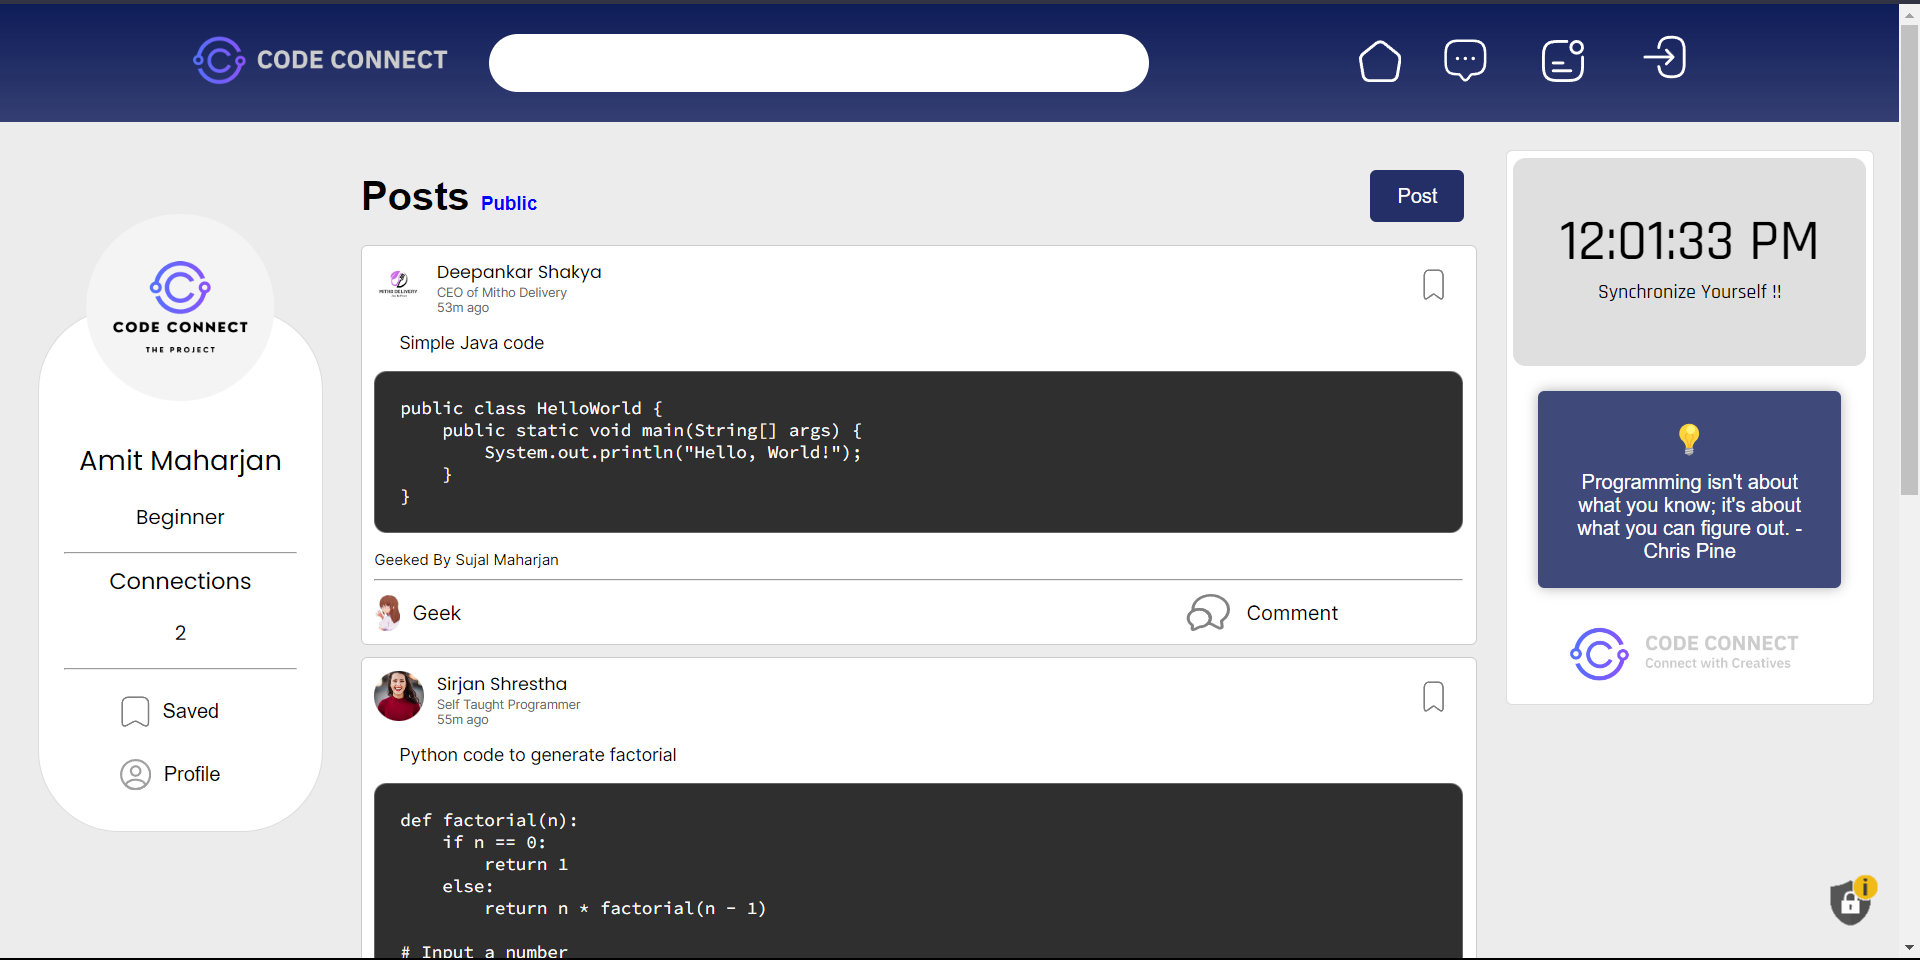
\includegraphics[height = 6.8cm]{Outcome-ss/homepage.png}
  \caption{Desktop Homepage UI}
\end{figure}
Below shows the UI Design of our Messenger System which have been implemented in our system.
\begin{figure}[H]
  \centering
  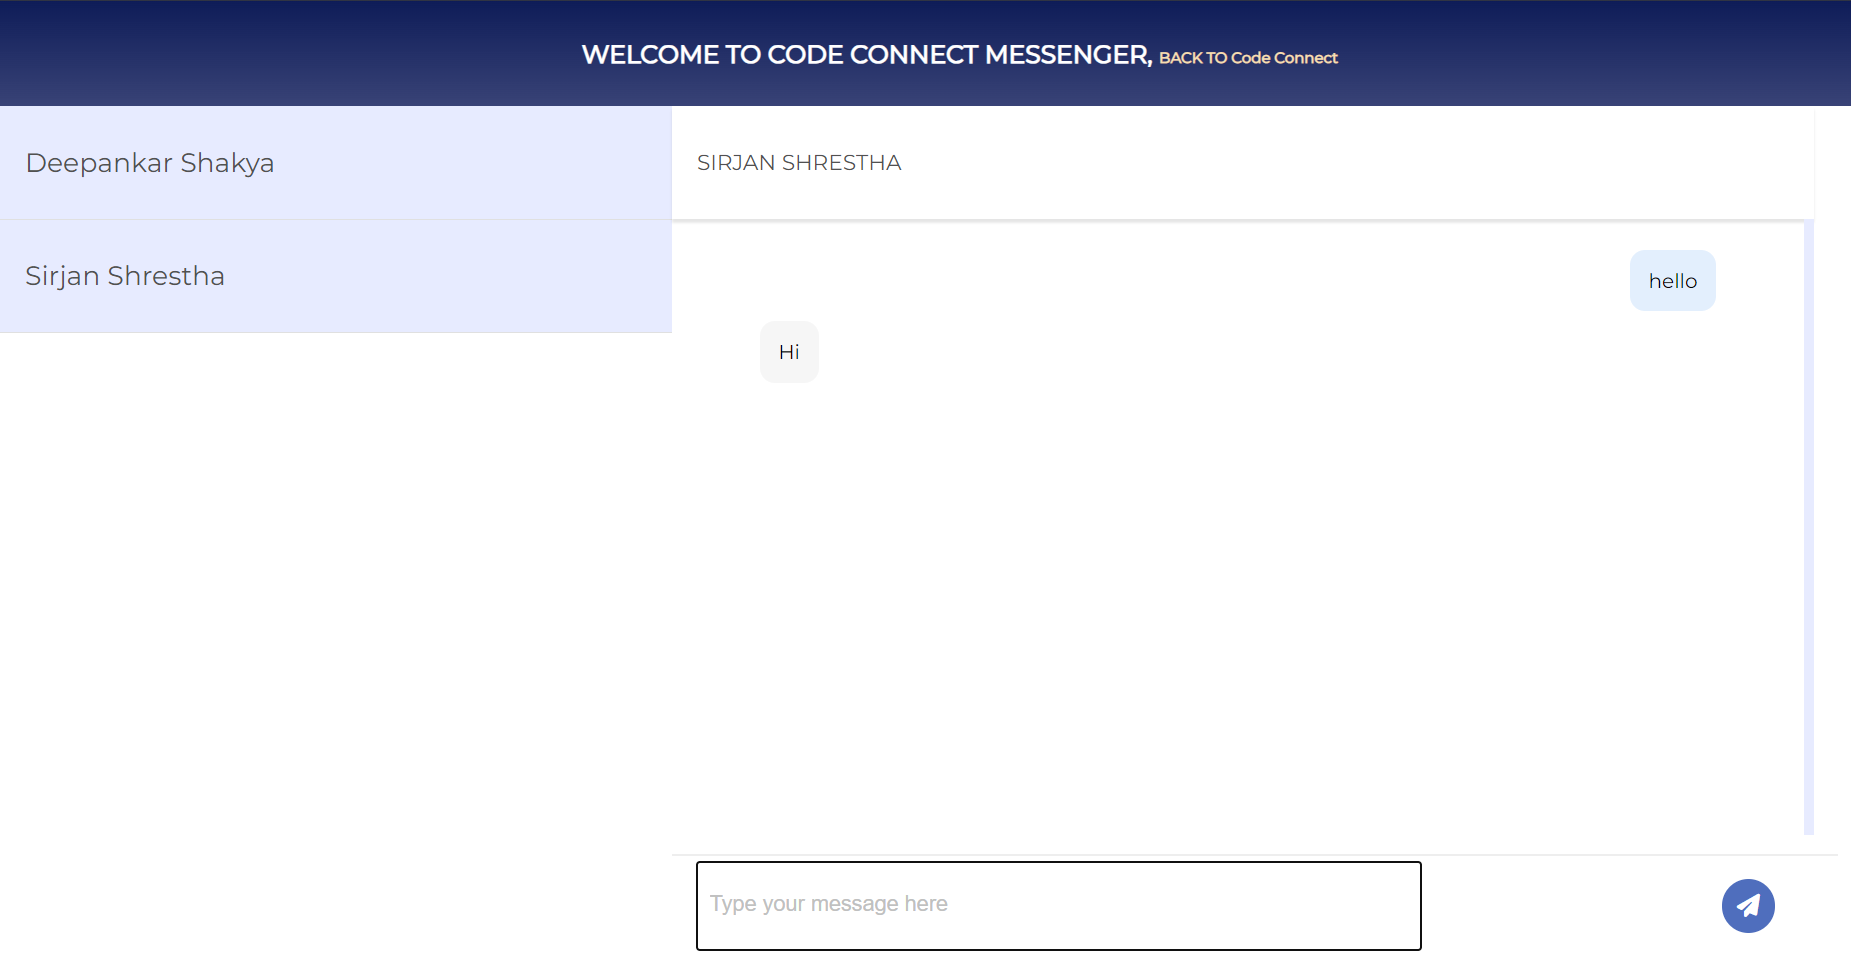
\includegraphics[height = 6.8cm]{Outcome-ss/messenger-full-block.png}
  \caption{Desktop Messages UI}
\end{figure}
\newpage
Below shows our Mobile Interface Login UI used in code connect.
\begin{figure}[H]
  \centering
  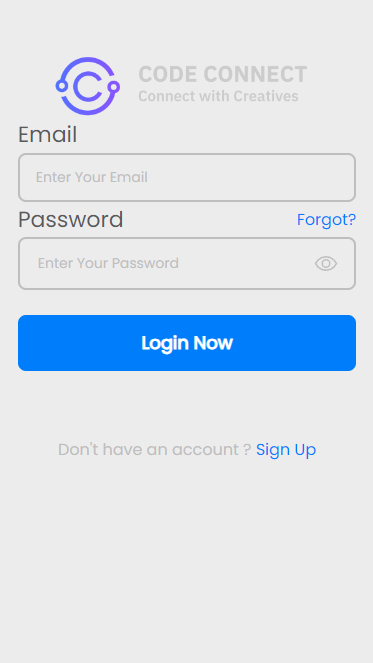
\includegraphics[height = 8cm]{ui_diagrams/mobile_login.png}
  \caption{Mobile Login UI}
\end{figure}

Below shows our Mobile Homepage UI used in code connect.
\begin{figure}[H]
  \centering
  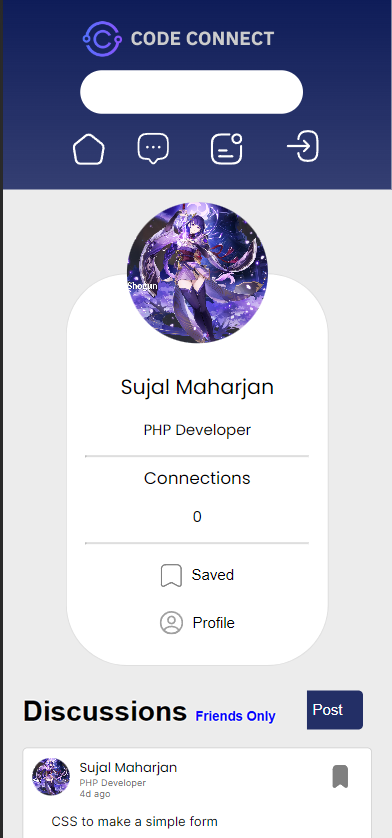
\includegraphics[height = 8cm]{Outcome-ss/mobile-homepage.png}
  \caption{Mobile Homepage UI}
\end{figure}

\newpage
Below shows our Mobile Chat UI used in code connect.
\begin{figure}[H]
  \centering
  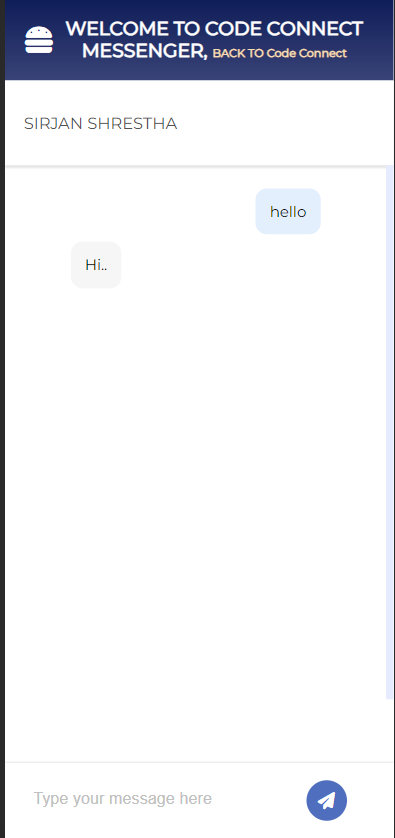
\includegraphics[height = 8cm]{Outcome-ss/mobile-chat.png}
  \caption{Mobile Chat UI}
\end{figure}

Below shows our Mobile Chat section's friend-list UI used in code connect.
\begin{figure}[H]
  \centering
  
\includegraphics[height = 8cm]{Outcome-ss/moble-chat-friends.png}
  \caption{Mobile Friend-list of chat UI}
\end{figure}

\subsection{Physical DFD}
A Physical Data Flow Diagram (DFD) is a graphical representation of how data flows within a system at a more detailed and implementation-oriented level than a logical DFD. While a logical DFD focuses on the system's functional aspects and processes, a physical DFD includes details about how data is processed, where it's stored, and how it's transferred between system components.

Here, main process Code Connect which is connected with other processes and sending and reviving data. There is user entity which initally react with Code Connect process and goes arround alll the processed.There is Data storage where processes store data and retrieve data as per their requirement.

\begin{figure}[H]
  \rotatebox{90}{
  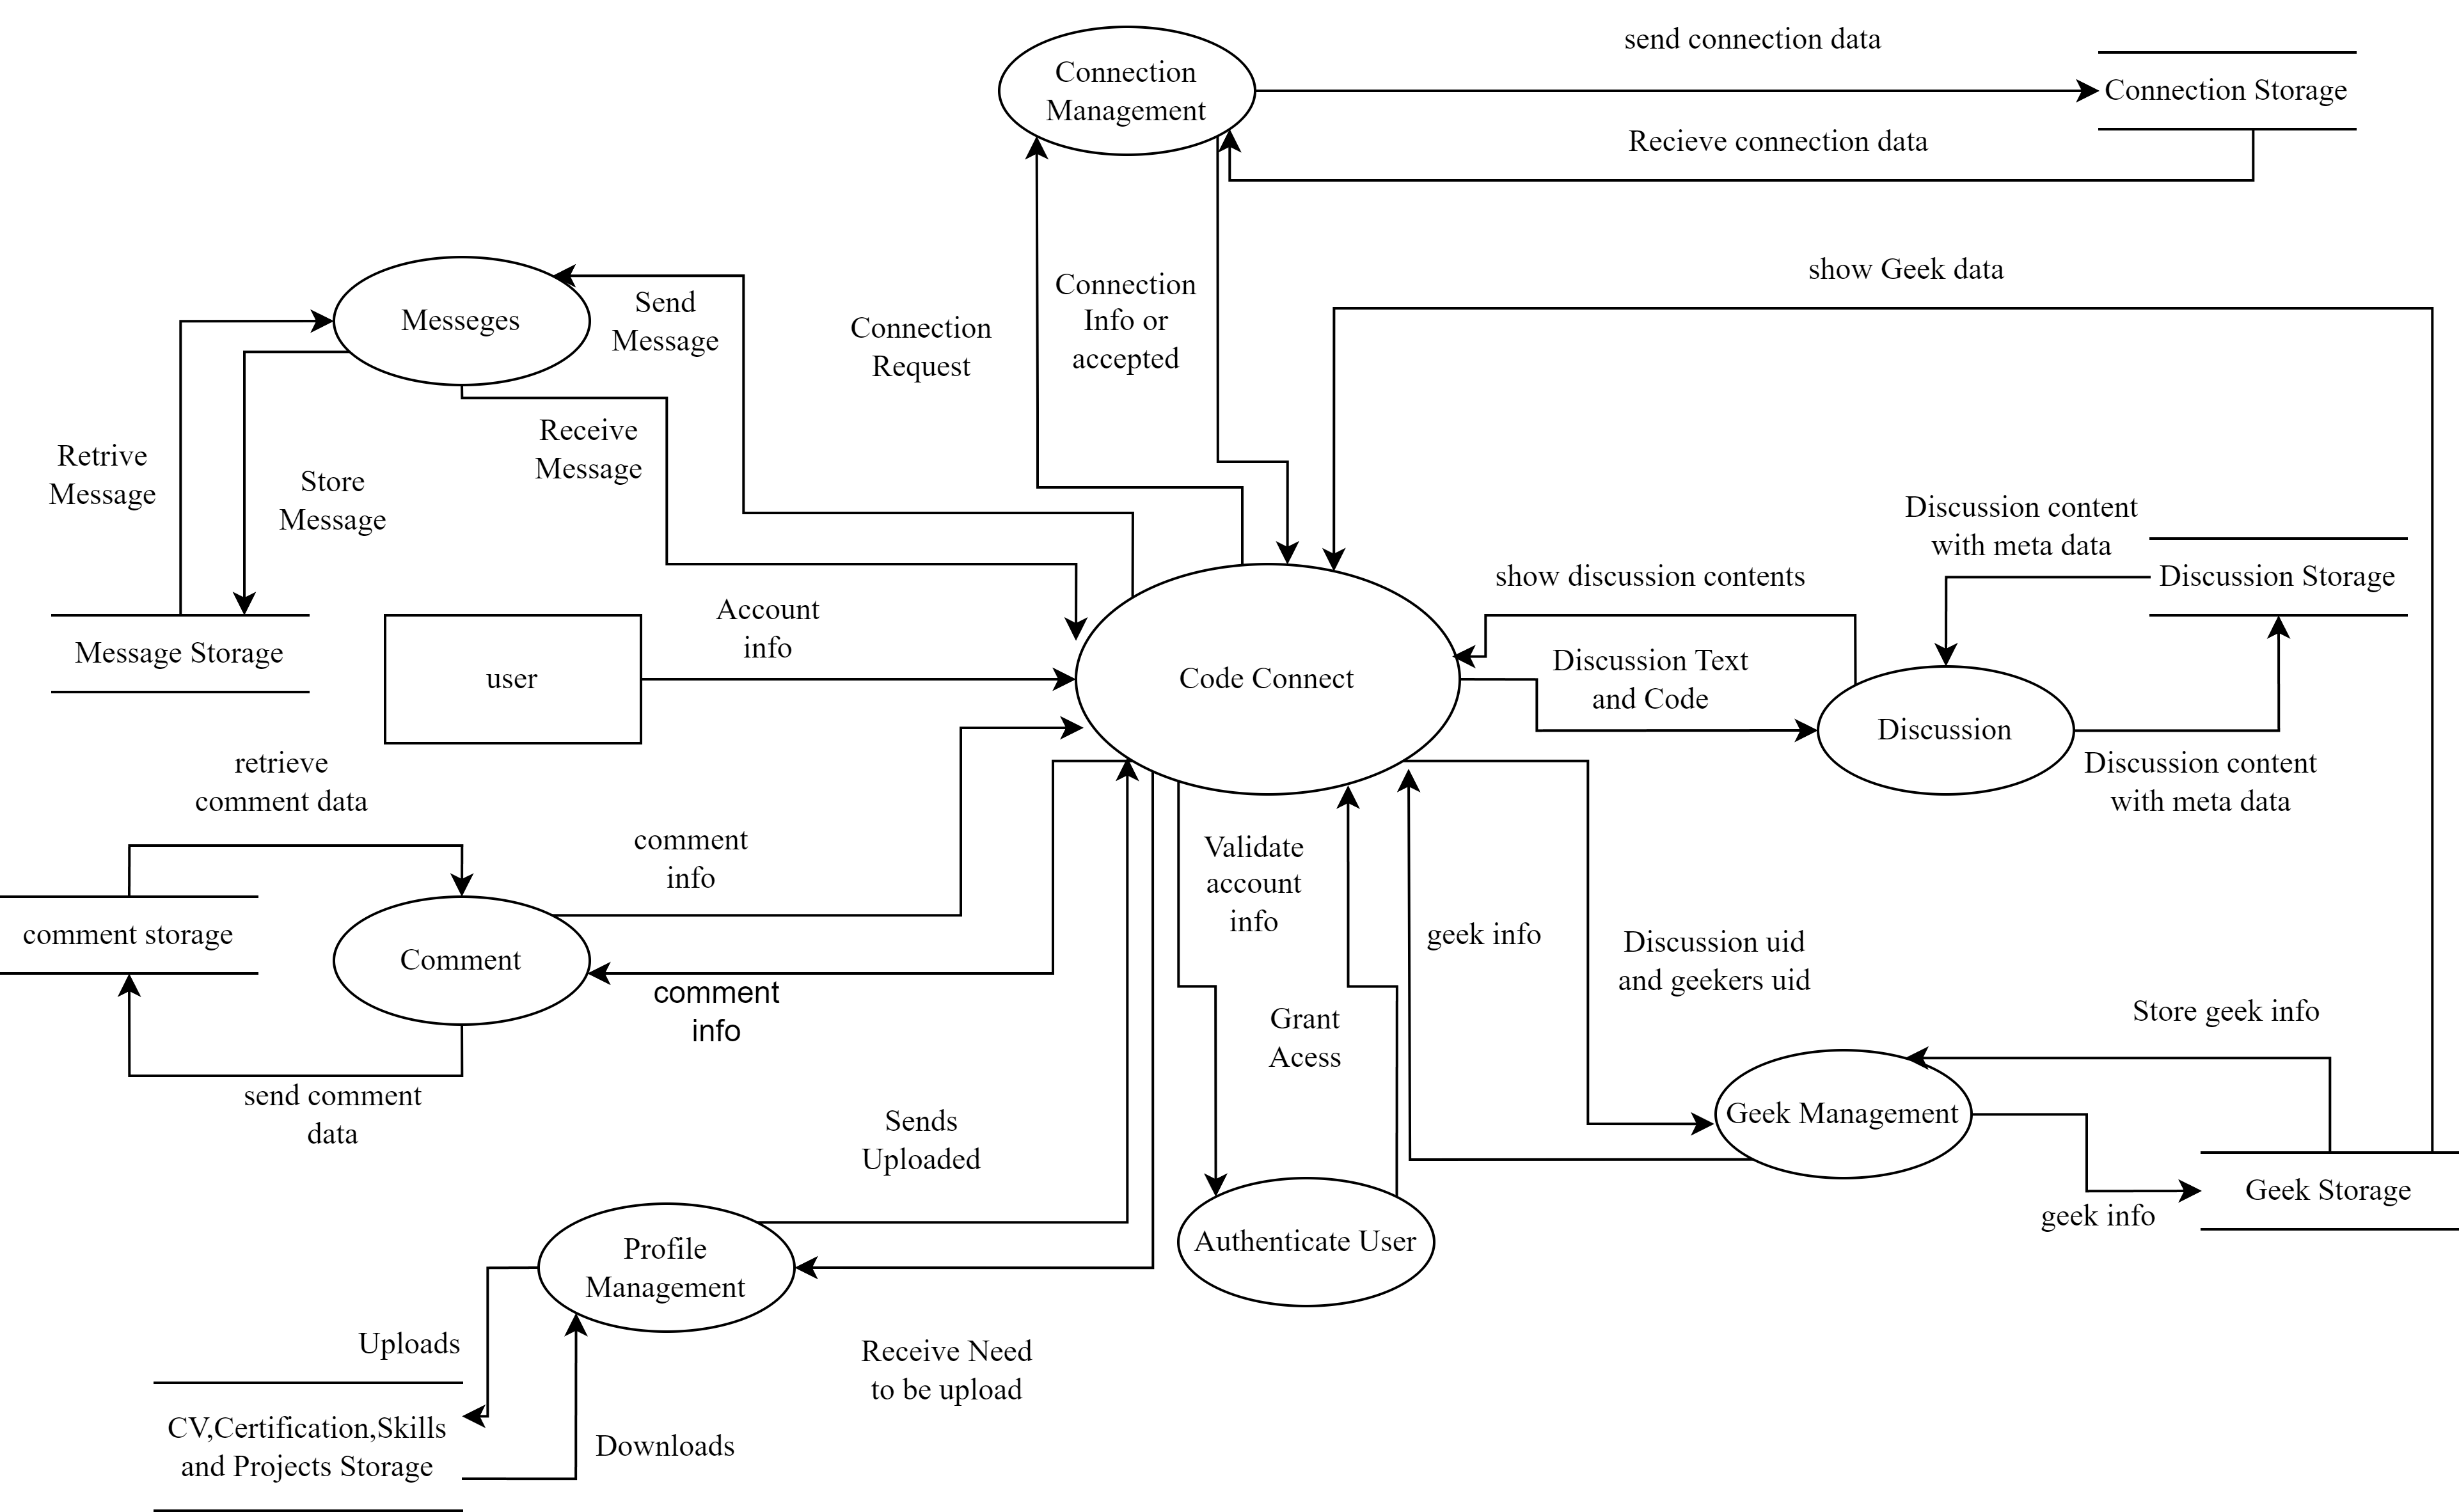
\includegraphics[height = 14cm]{Diagrams/physical_dfd.png}}
  \caption{Physical DFD of System}
\end{figure}
\newpage